%% ---------------------------------------------------------------------------------
\begin{frame}
  \titlepage
\end{frame}
%% ---------------------------------------------------------------------------------

%%%% ---------------------------------------------------------------------------------
\begin{frame}[c] \frametitle{Overview}
%  \framesubtitle{Untertitel}
  \begin{itemize} \setlength{\itemsep}{18pt}
    \item Introduction
    \item Problems with existing solutions
    \item Our solution
    \item Demo
  \end{itemize}
\end{frame}
%%%% ---------------------------------------------------------------------------------

\section{Introduction}
\sectionpage

%%%% ---------------------------------------------------------------------------------
%%%% Introduction
%%%% ---------------------------------------------------------------------------------
\begin{frame}[t]\frametitle{Introduction}
 \framesubtitle{What is remote signing?}
 \begin{columns}[T]
	\begin{column}{0.5\textwidth}
		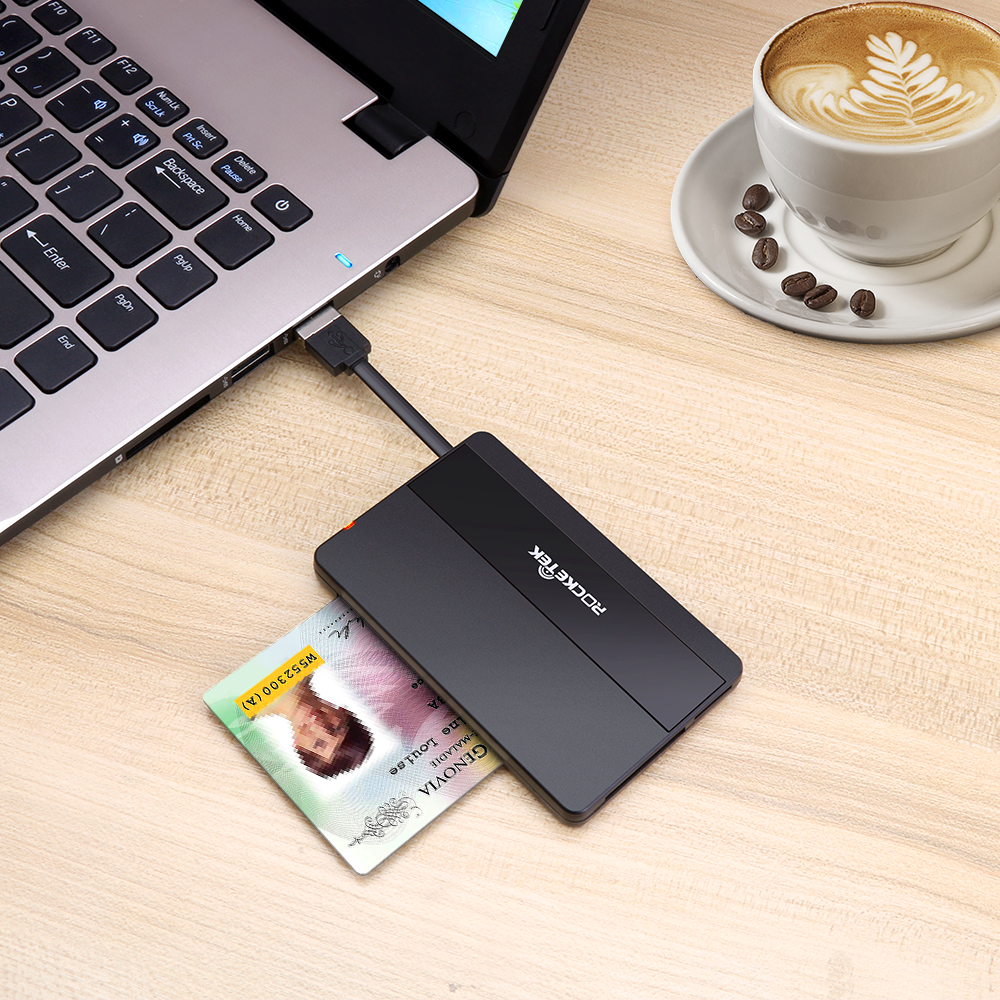
\includegraphics[width=\textwidth]{cardreader.jpg}
	\end{column}
	\begin{column}{0.5\textwidth}
		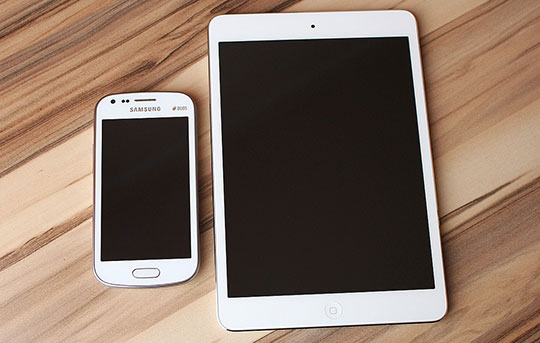
\includegraphics[width=\textwidth]{tablet-smartphone.jpg}
	\end{column}
 \end{columns}
\end{frame}

\begin{frame}[t]\frametitle{Introduction}
 \framesubtitle{What is remote signing?}
  \begin{itemize}
    \item Electronic signatures
    \begin{itemize}
      \item are legally binding
	  \item use digital signatures (cryptographic primitives)
    \end{itemize}
    \item No more hardware tokens
    \item Signing from every device, everywhere
    \item Signature Activation Protocol for unlocking the private key
  \end{itemize}
\end{frame}
%%%% ---------------------------------------------------------------------------------

\section{Problems with existing solutions}
\sectionpage


\begin{frame}[t]\frametitle{Problems with existing solutions}
	\framesubtitle{Adobe Sign}
	\begin{itemize}
	  \item Users don't have control of their private keys
      \item Signing Service can create signatures without the User's knowledge
      \item Implementation of Signature Activation Protocol is trust based
      \item Has access to your documents
	  \item Based on CSC standard, but implementation is proprietary
	  \item (over 200 Identity providers (who is the authoritative source))
	  \item Only possible to sign PDFs
	\end{itemize}
\end{frame}


\section{Our Solution}
\sectionpage

\begin{frame}[t]\frametitle{Our Solution}
	\framesubtitle{Overview}
	\begin{itemize}
		\item Trust is distributed between IdP and Signing Service
		\item Sign arbitrary documents
		\item Signing Service only receives hash of document
		\item Web-Based
		\item Signature Activation Protocol is based on cryptography
		\item Offline verification
	\end{itemize}
\end{frame}

\begin{frame}[t]\frametitle{Our Solution}
	\framesubtitle{How we do it}
	\begin{itemize}
		\item Reuse the Nonce in the OIDC ID token
		\begin{itemize}
			\item nonce consists of list of salted hashes of the documents
			\item couples documents with the ID token
		\end{itemize}
		\item Signing Service can only sign the hashes which flow into the nonce
		\item Signature is detached (separate file)
		\item All certificate chains and revocation info(crl/ocsp) are in the signature for offline verification
	\end{itemize}
\end{frame}

%%%% ---------------------------------------------------------------------------------
%%%% Important Websites
%%%% ---------------------------------------------------------------------------------
\begin{frame}[c]\frametitle{Important Websites at BFH}
  \framesubtitle{Access your data, send e-mails and change the personal password}
  \begin{block}{Intranet}
    \url{https://intranet.bfh.ch}
  \end{block}
  \begin{alertblock}{Webmail}
    \url{https://webmail.bfh.ch}
  \end{alertblock}
  \begin{block}{Module List}
    \url{https://is-a.bfh.ch}
  \end{block}
  \begin{alertblock}{PWD, BFH-Card, E-Mail redirect}
    \url{https://selfhelp.bfh.ch}
  \end{alertblock}
  \begin{block}{E-Learning}
    \url{https://moodle.bfh.ch}
  \end{block}
\end{frame}
%%%% ---------------------------------------------------------------------------------

\part{GAGA}

\partpage

%%%% ---------------------------------------------------------------------------------
%%%%  Where to get software? Where to buy hardware
%%%% ---------------------------------------------------------------------------------
\begin{frame}[t]\frametitle{Special offer for software/hardware purchase}

  \begin{columns}[c]
  \begin{column}{0.5\textwidth}
     \begin{figure}[ht]
     \centering
     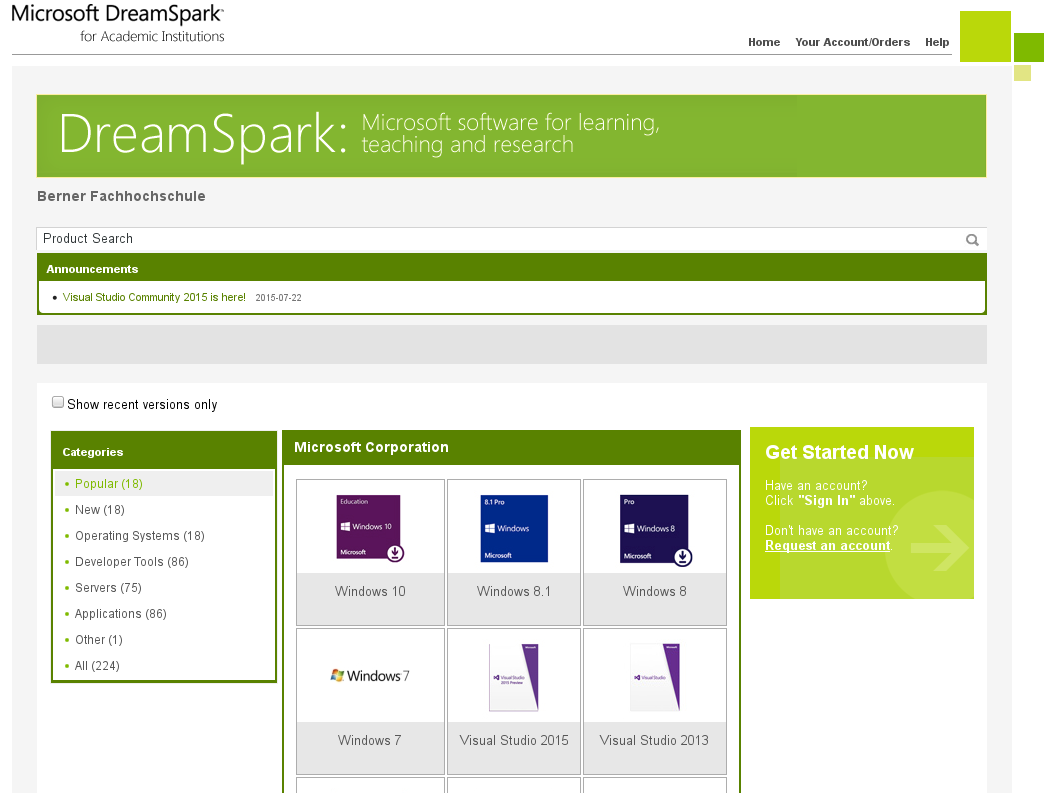
\includegraphics[width=\textwidth]{offers-software}
     \end{figure}
  \end{column}
  \begin{column}{0.54\textwidth}
     \begin{figure}[ht]
     \centering
     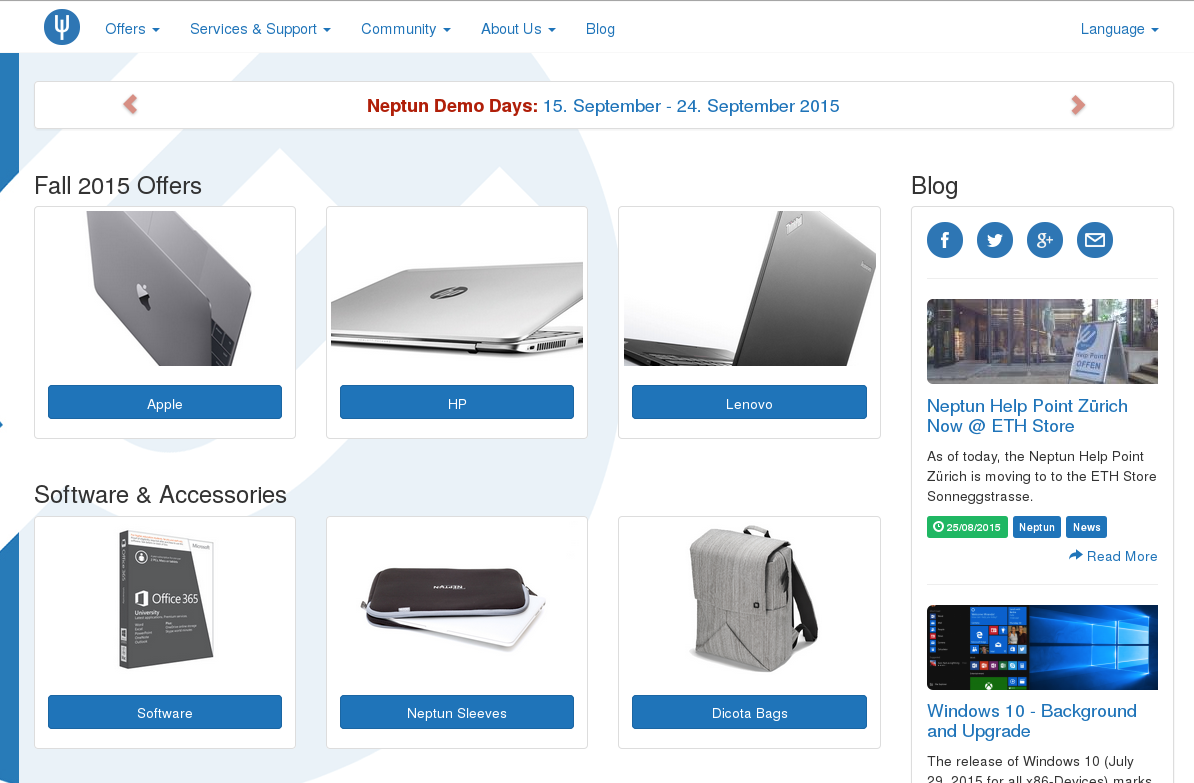
\includegraphics[width=\textwidth]{offers-hardware}
     \end{figure}
  \end{column}
  \end{columns}
  
  \vskip3em
  For a more detailed description follow the link below:
  
  \begin{itemize}
    \item<2-> \url{https://gtilab.ti.bfh.ch}
  \end{itemize}

\end{frame}
%%%% ---------------------------------------------------------------------------------

\subsection{bla bla}

\subsectionpage

%%%% ---------------------------------------------------------------------------------
\begin{frame} \frametitle{What are the minimal HW requirements}
  \begin{itemize}\setlength{\itemsep}{10pt}
  \item<1-> As a student in an engineering department you have to bring a laptop \textit{(price around 1k)}
  \item<2-> For computer science and electronics courses the following minimal settings are sufficient:
    \begin{multicols}{2}
      \begin{itemize}\setlength{\itemsep}{5pt}
        \item CPU : Intel Core i5
        \item RAM : 8GB
        \item SSD : $\geq$256GB 
        \item Intel HD Graphics
        \item For CAD Nvidia GForce 
        \item Size: 13", 14" or 15"
        \item Features : VT-x (+ VT-d)
      \end{itemize}
    \end{multicols}
    \item<3-> \url{https://www-ssl.intel.com/content/www/us/en/processors/processor-numbers.html}
  \end{itemize}
\end{frame}
%%%% ---------------------------------------------------------------------------------
